\def\year{2016}\relax
%File: formatting-instruction.tex
\documentclass[letterpaper]{article}
\usepackage{aaai16}
\usepackage{times}
\usepackage{helvet}
\usepackage{courier}
\usepackage{graphicx}
\usepackage{subcaption}
\usepackage{tikz}
\usepackage{todonotes}
\usepackage{enumitem}
\def\checkmark{\tikz\fill[scale=0.4](0,.35) -- (.25,0) -- (1,.7) -- (.25,.15) -- cycle;} 

\frenchspacing
\setlength{\pdfpagewidth}{8.5in}
\setlength{\pdfpageheight}{11in}

\pdfinfo{
/Title (CRQA: Crowd-powered Real-time Automated Question Answering System)
/Author (Denis Savenkov, Eugene Agichtein)}
\setcounter{secnumdepth}{0}  
 \begin{document}
% The file aaai.sty is the style file for AAAI Press 
% proceedings, working notes, and technical reports.
%
\title{CRQA: Crowd-powered Real-time Automated Question Answering System}
\author{
	Denis Savenkov\\
	Emory University\\
	\texttt{dsavenk@emory.edu}
\And
	Eugene Agichtein\\
	Emory University\\
	\texttt{eugene@mathcs.emory.edu}
}

\maketitle
\begin{abstract}
Modern search engines have made dramatic progress in the answering of questions about facts, such as those that might be retrieved or directly inferred from a knowledge base.
However, many other questions that real users ask are more complex, such as requests for opinions or advice for a particular situation, and are still largely beyond the competence of the computer systems.
As conversational agents become more popular, QA systems are increasingly expected to handle such complex questions, and to do so in (nearly) real-time, as the searcher is unlikely to wait longer than a minute or two for an answer.
One way to overcome some of the challenges in complex question answering is crowdsourcing.
We explore two ways crowdsourcing can assist a question answering system that operates in (near) real time: by providing answer {\em validation}, which could be used to filter or re-rank the candidate answers, and by {\em creating} the answer candidates directly.
In this paper we present CRQA, a crowd-powered, near real-time automated question answering system for complex informational tasks, that incorporates a crowdsourcing module for augmenting and validating the candidate answers.
The crowd input, obtained in real-time, is integrated into CRQA via a learning-to-rank model, to select the final system answer.
Our large-scale experiments, performed on a live stream of real users questions, show that even within a one minute time limit, CRQA can produce answers of high quality.
The returned answers are judged to be significantly better compared to automated system alone, and even are often preferred to answers posted days later in the original community question answering site.
Our findings can be useful for developing hybrid human-computer systems for automatic question answering and conversational agents.
\end{abstract}

\section{Introduction}
\label{sec:introduction}
It has long been a dream to communicate with a computer as one might with another human being using natural language speech and text.
We are now coming closer to this dream, as natural language interfaces become increasingly popular.
Our phones are already reasonably good at recognizing speech, and personal assistants, such as Apple Siri, Google Now, Microsoft Cortana, Amazon Alexa, \textit{etc.}, help us with everyday tasks and answer some of our questions.
Chat bots are arguably considered ``the next big thing'', and a number of startups developing this kind of technology has emerged in Silicon Valley and around the world\footnote{http://time.com/4194063/chatbots-facebook-messenger-kik-wechat/}.

Question answering is one of the major components of such personal assistants.
Existing techniques already allow users to get direct answers to their factoid questions.
%\footnote{https://www.stonetemple.com/rich-answers-in-search/}.
However, there is still a large number of more complex questions, such as advice or accepted general opinions, for which users have to dig into the ``10 blue links'' and extract or synthesize answers from information buried within the retrieved documents.
To cater to these informational needs, community question answering (CQA) sites emerged, such as Yahoo! Answers and Stack Exchange.
These sites provide a popular way to connect information seekers with answerers.
Unfortunately, it can take minutes or hours, and sometimes days, for the community to respond, and some questions are left unanswered altogether. 

To facilitate research on this challenge, TREC LiveQA shared task\footnote{http://www.trec-liveqa.org} was started in 2015, where automated systems attempt to answer real users' questions within a 1 minute period.
This task was successful, with the winning system able to automatically return a reasonable answer to more than half of the submitted questions, as assessed for TREC by the trained judges from NIST.
Nevertheless, many questions were not answered well by any of the participating systems.

In this work we explore two ways \textit{crowdsourcing} can be used to help an automated system answer complex user questions.
The main challenge is how to adapt existing ``batch-mode'' crowdsourcing platforms such as Amazon Mechanical Turk to real-time settings, \textit{e.g.}, to produce an answer within a minute.
More specifically, our research questions can be stated as:
\textbf{RQ1}. Can crowdsourcing be used to improve the performance of a near real-time automated question answering system?
\textbf{RQ2}. What is the relative contribution of candidate answer ratings and answers provided by the workers to the overall question answering performance?
\textbf{RQ3}. What are the trade-offs in performance, cost, and scalability of using crowdsourcing for real-time question answering?

To explore these research questions, we introduce our CRQA system, which stands for Crowd-powered Real-time Question Answering.
CRQA integrates a crowdsourcing module into an automated question answering system within an overall learning-to-rank framework for selecting answers to complex questions.
We report extensive experiments of stress-testing the CRQA system, by participating in the TREC LiveQA 2016 evaluation challenge, which provided us with a realistic evaluation setup.

Specifically, the contributions of this paper are threefold:
\begin{enumerate}
	\item CRQA, a novel hybrid near real-time question answering system, that uses crowd workers to rate and augment automatically generated candidate answers.
	\item Large scale experiments using CRQA to answer real user questions in a live TREC LiveQA 2016 challenge setting.
	\item Extensive analysis of the system performance, focusing on the contributions of crowd input to the performance of the overall system.
\end{enumerate}

The results and findings of this work can be useful to guide future research on hybrid human-computer question answering, and automated intelligent assistant systems.

\section{System design}
\label{sec:system}

Before diving into the architecture of our Crowd-powered Real-time Question Answering (CRQA) system, we will describe the setup of the TREC LiveQA 2016 shared task, which affected some of the system design choices.

A series of TREC LiveQA evaluation campaigns was started in 2015 with the goal to facilitate research in automatic question answering for complex informational needs.
A good overview of the shared task and last years results can be found in \cite{agichtein2015overview}.
In TREC LiveQA'16 shared task participants are to develop a question answering system to answer real user questions, which are sampled from a live stream of questions posted to Yahoo! Answers community question answering (CQA) website, and do that in under a one minute time limit.
Each question consists of the short question title, question body and category.
As a response systems need to provide an answer of up to 1000 characters long, generated from any available data source.

Our CRQA system represents a hybrid system, that includes an automated question answering and crowdsourcing modules.
The high level architecture is presented in Figure~\ref{fig:system}.

\begin{figure*}[h!t]
	\centering
	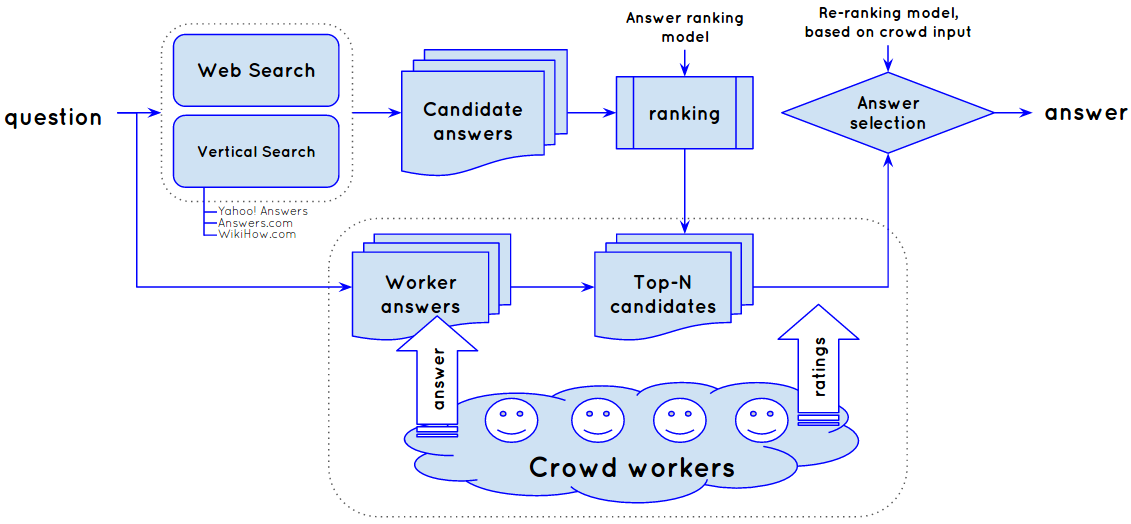
\includegraphics[width=\textwidth]{img/system}
	\caption{The architecture of our Crowd-powered Real-time Question Answering system, that uses crowdsourcing to augment a list of automatically extracted candidate answers and to rate their quality}
	\label{fig:system}
\end{figure*}

The automated part of the CRQA system follows an Information Retrieval (IR) approach to question answering, and generates a set of candidate answer passages from multiple data sources.
After candidates are generated, they are ranked by a trained model, and in the fully automated mode the top candidate could be returned as the answer.
The crowdsourcing module is designed to overcome two of the most common problems of the automated QA approaches: lack of good candidate answers and ranking errors.
More particularly, CRQA asks crowd workers to provide answers to the given questions if they can, and additionally rate the quality of candidate answers, generated by the automated system.
Worker contributions are then used by a trained re-ranking model, that selects the best candidate answers using all the information available.
The next two sections describe the architectures of the automated and crowdsourcing modules of our system.

\subsection{Automated question answering module}
\label{sec:system:auto}

When CRQA receives a question, it generates a set of search queries to retrieve a set of relevant documents and extract candidate answer passages.
Search queries are generated using the following strategies:
\begin{itemize}
\item Question title, which most often captures the gist of the question
\item Two longest question sentences (detected by the presence of the question word at the beginning or question mark at the end of a sentence) from the title and body of the question. In some cases the real user question is hidden inside the body, while the title just provides the overall topic of the question.
\item Concatenation of the question word, verbs and top-5 terms from the question title by Inverse Document Frequency\footnote{IDF of terms are estimated using Google N-gram corpus: https://catalog.ldc.upenn.edu/LDC2006T13}. This strategy targets over-specific questions, which often retrieve few if any search results.
\end{itemize}

To retrieve a set of potentially relevant documents and extract candidate answer passages, CRQA relies on multiple different generic and CQA document collections.
Previous research \cite{shtok2012learning} has shown that many of the user information needs are repeated, and reusing answers to previously posted similar questions is an effective strategy for answering new questions.
Therefore, CRQA uses multiple different CQA data sources, which potentially contain a diverse set of questions.
However, quite often it is hard to find a similar question in an archive, and many of the information needs are unique.
Therefore, we include a web search component, that can retrieve regular web documents, from which our system can extract candidate answers.
More specifically, CRQA queries the web using Bing Web Search API\footnote{https://datamarket.azure.com/dataset/bing/searchweb}, Yahoo! Answers, Answers.com and WikiHow.com using their respective search interfaces.
For each query we retrieve top-10 relevant documents and question-answer pairs from CQA archives.
As candidate answers CRQA extracts answers to the questions retrieved from CQA results and paragraphs of text from the main content of regular web documents, as detected by a method based on \cite{Kohlschutter_2010}.
Quite often, it's hard to estimate the quality of a candidate answers from its text only.
The task becomes much easier if a system has access to additional data, \textit{e.g.} for the candidates generated from the CQA archives, it is useful to know the text of the original question the candidate answers.
For candidates, generated from regular web pages, it's useful to know the topic of the page (\textit{e.g.} from its title), additionally the context of the candidate, such as text that immediately precedes it in the document was shown to provide a useful information for QA.
Therefore, besides the text of a candidate answer, we keep some potentially useful metadata, \textit{e.g.,} for QnA candidates we include text and category of the retrieved question, and web page title and text block preceding the answer passage in the document for web-search based candidates.
For convenience, we will call the title of a retrieved question or web page \textit{``the answer topic''}, and the body of the retrieved question or the preceding text block the \textit{``the answer context''}.

Next, for each candidate answer we compute a set of features, described in Table \ref{table:features}.

\begin{table}[ht]
\centering
\begin{tabular}{| p{8cm} |}
\hline
\textbf{Answer statistics} \\
\hline
--- Length in chars, words and sentences \\
--- Average number of words per sentence \\
--- Fraction of non-alphanumeric characters  \\
--- Number of question marks \\
--- Number of verbs  \\
\hline
\textbf{Answer source} \\
\hline
--- Binary feature for each of the search verticals: Web, Yahoo! Answers, Answers.com, WikiHow.com \\
\hline
\textbf{N-gram matches}\\
\hline
--- Cosine similarities using uni-, bi- and tri-gram representations of the question title and/or body, and answer text, topic or context\\
--- The lengths of longest spans of matched terms between question title and/or body, and answer text, topic or context\\
\hline
\textbf{Information Retrieval score}\\
\hline
--- BM25 scores between question title and/or body, and answer text, topic or context\\ 
\hline
\end{tabular}
\caption{The list of candidate answer ranking features used by the automated module of our CRQA system}
\label{table:features}
\end{table}

The final stage of the module is answer ranking, where a trained LambdaMART \cite{burges2010ranknet} model sorts the candidates by their predicted quality.
This model was trained using the RankLib library\footnote{https://sourceforge.net/p/lemur/wiki/RankLib/} on the data from last year TREC LiveQA task\footnote{https://sites.google.com/site/trecliveqa2016/liveqa-qrels-2015}, which includes 1087 questions with answers provided by the participants, each of which was rated on a scale from 1(bad) to 4(excellent) by professional NIST assessors.
In a fully automated setup the top candidate could be returned as the final answer to the question, but in this work we explore if we can further improve the performance of the system using crowdsourcing.

\subsection{Crowdsourcing module}
\label{sec:system:crowd}

As we mentioned before, two of the main problems with the fully automated system responses are lack of good candidates and problems with ranking, therefore, we decided to explore if crowdsourcing can be helpful to overcome these challenges in near real-time scenario.
Instead of returning the final answer, the system sends the question and top-7 ranked candidates to the crowd workers and waits for the responses.
We chose to give 7 answers based on the average number of rated answers in our preliminary studies.
Since systems had only 60 seconds to answer each question, we start a timer when a question arrives, and the system waits to receive all worker contributions until the timer reaches 50 seconds to leave the system some time to generate the final answer and minimize the chances of going above the time limit.
CRQA asks workers to write their own answers to questions if possible, which should provide additional candidates in case there are no good automatically generated ones.
Additionally, systems expects workers to rate the quality of top-7 ranked candidates, which should help to fix the ranking problems and select a better final answer.
Figure~\ref{fig:crowd_ui} presents the user interface of our crowdsourcing module.

\begin{figure*}[h!t]
	\centering
	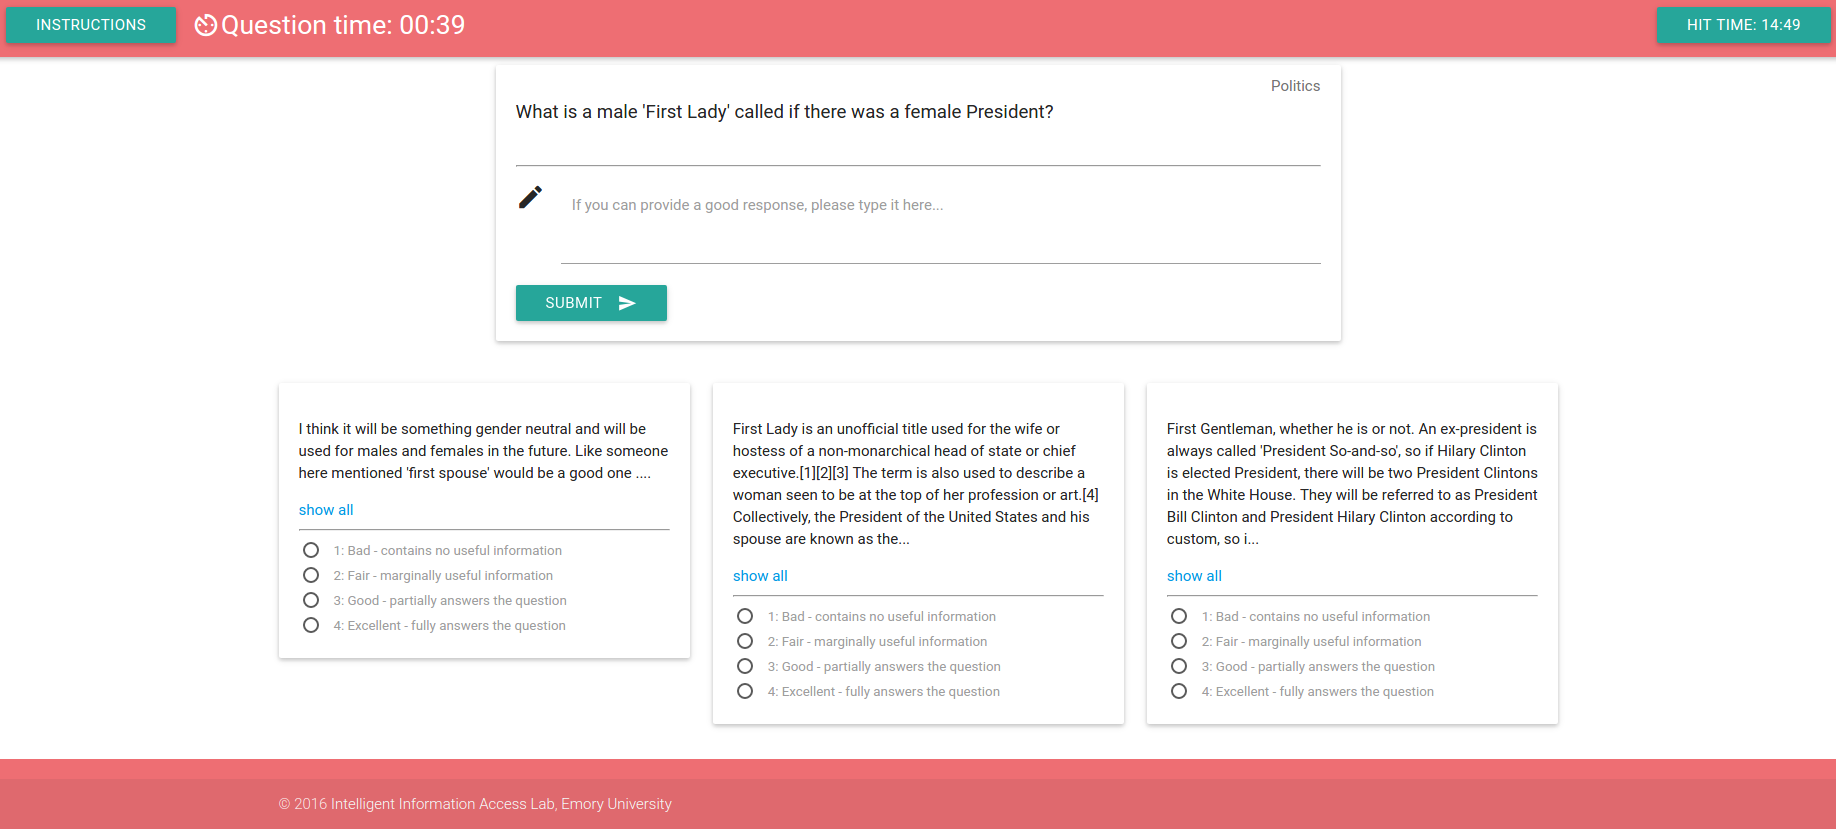
\includegraphics[width=\textwidth]{img/crowd_ui}
	\caption{User Interface for workers in our Crowd-Powered Question Answering system}
	\label{fig:crowd_ui}
\end{figure*}

The overall algorithm for obtaining crowd input for real-time question answering is the following:
\begin{enumerate}
\item When a system receives a question, it is posted to the workers, who will have 50 seconds to provide their input
\item Workers are asked to write an answer if they can provide one (it's optional)
\item Otherwise they are waiting for the answer candidates to arrive
\item When a system is done with generating and ranking candidates it posts top-7 scoring answers to the workers for the rating (which usually leaves $\sim$ 35 seconds for rating)
\item Workers receive a list of answers\footnote{Answers submitted by workers are also sent for ratings to all workers except the author} and rate them until the timer runs off. Each answer is rated on a scale from 1 to 4, using the official TREC LiveQA rating scale:
	\begin{itemize}[noitemsep,topsep=0pt]
    \item 1 --- Bad: contains no useful information
    \item 2 --- Fair: marginally useful information
    \item 3 --- Good: partially answers the question
    \item 4 --- Excellent: fully answers the question
    \end{itemize}
\item The interface displays 3 answers at a time, when an answer gets rated, it disappears and its place is taken by another answer from the pool. The interface displays only the first 300 characters of the answer, which was experimentally shown to be enough on average to make a good judgment.
Full answer can be revealed upon clicking the ``show all'' link.
\item When the timer runs off, the question and all the answers disappear, and workers wait for the next question
\end{enumerate}

% Not sure we need a title, as this subsection already describes the crowdsourcing module.
% \noindent\textbf{QARC system implementation: Crowd module}:
To hire the workers we used Amazon Mechanical Turk platform\footnote{http://mturk.com}.
Since the challenge was to run the system ``live'' over the period of 24 hours, we adapted the ``retainer'' model to our question-answering task, inspired by the success of this model reported in previous work \cite{bernstein2011crowds,bigham2010vizwiz}.
Specifically, to obtain an even distribution of workers over the 24-hour period of the TREC LiveQA shared task, we posted 10 tasks every 15 minutes, and they expired after the next set of tasks became available.
Since not all assignments were accepted by some worker right away, the number of workers for each question varied and could be greater than 10.
% This seems to be out of context, as we didn't tell how many questions we had, etc.
% In total there were 960 tasks posted to Amazon Mechanical Turk, from which 889 were completed successfully within the allotted time of 1 minute.
When a worker first gets to our crowdsourcing interface, she is shown task instructions (Table \ref{table:crowd_instructions}) and asked to wait for the questions to arrive.
The workers were paid \$1.00 for the whole 15 minutes task, no matter how many questions they got\footnote{In TREC LiveQA task questions are sent to the systems one by one, therefore there is no concurrency, however the delays between the questions are possible}.

\begin{table}[ht]
\centering
\begin{tabular}{| p{8cm} |}
\hline
\textbf{Instructions} \\
\hline
1. This HIT will last exactly 15 minutes\\
2. Your HIT will only be submitted after these 15 minutes\\
3. In this period of time you will receive some questions, that came from real users on the Internet\\
4. Each question has a time limit after which it will disappear and you will need to want for the next one\\
5. If you know the answer to the question, please type it in the corresponding box\\
6. At some point several candidate answers will appear at the bottom of the page\\
7. Please rate them on a scale from 1 (bad) to 4 (excellent)\\
8. Do not close the browser or reload the page as this will reset your assignment.\\
\hline
\end{tabular}
\caption{Crowdsourcing task instructions, displayed to the user when she first gets to the task}
\label{table:crowd_instructions}
\end{table}

\subsection{Answer re-ranking and selection}
\label{sec:system:reranking}

The last stage in CRQA is answer re-ranking, which aggregates all the information received from the crowdsourcing and produces the final answer to the question.
The input of the re-ranking module is a set of candidate answers with quality ratings provided by the crowd workers.
Candidates can include the answers posted by the workers, which might also be rated, if workers had enough time to do that.
To re-rank the answers we trained a gradient boosting regression trees (GBRT) model \cite{friedman2002stochastic}.
To build this model we used a training set of questions with answers generated by our system.
The quality of each answer was manually assessed using the official LiveQA scale from 1 (bad) to 4 (excellent).
The features, used for answer re-ranking are listed in Table \ref{table:reranking_features}.

\begin{table}[ht]
\centering
\begin{tabular}{| p{8cm} |}
\hline
\textbf{Answer-based} \\
\hline
--- The length of the answer \\
--- Source of the answer (Crowd, Web, Yahoo! Answers, Answers.com or WikiHow.com)\\
--- Original rank of the candidate answer or -1 for answers provided by the crowd workers\\
\hline
\textbf{Worker ratings} \\
\hline
--- Number of ratings provided\\
--- Minimum, maximum, median and average ratings\\
\hline
\end{tabular}
\caption{The list of features used for answer re-ranking based on crowdsourcing input}
\label{table:reranking_features}
\end{table}

CRQA sorts the candidates by the quality score predicted by the model, as returns the top candidate as the final answer.



\section{Experiments}
\label{sec:experiments}
We now describe the experimental setup used to evaluate the performance of CRQA and other methods for near real-time question answering.

\subsection{Experimental Setup: TREC LiveQA}
The experimental evaluation of our CRQA system was done on the official run of TREC LiveQA shared task, which happened on May 31, 2016.
All participating systems were running for 24 hours and received questions sampled from the live (real time) stream of questions, posted by real users to Yahoo! Answers platform.
In total, each system received 1,088 questions, and system responses were recorded by the organizers.

\begin{table}[ht]
\centering
\begin{tabular}{| p{7cm} | c | }
\hline
Name & Value \\
\hline
Number of questions received & 1088 \\
Number of completed assignments (15 mins each) & 889 \\
Average number of questions per assignment & 11.44 \\
Total cost per question & \$0.81 \\
Average number of answers provided by workers & 1.25 \\
Average number of ratings per answer & 6.25 \\
\hline
\end{tabular}
\caption{Aggregate statistics of crowdsourcing tasks}
\label{table:task_stats}
\end{table}

Overall statistics are provided in Table \ref{table:task_stats}.
As we can see, on average workers were able to provide at least one answer for each question, and each of the provided answers got 6 ratings.
Since the interface could show only 3 answers at a time, answers had different chances of being rated.
To investigate the effect of the order of the candidates posted for ratings on the quality of the final answer, in CRQA for each worker and each question we randomly selected one of the strategies: ordering answer candidates by their model rank or random shuffling of the candidates.
The system variant with shuffled candidates for rating was expected to obtain more diverse and comprehensive set of ratings, as we will investigate in the Analysis section.

\subsection{Answer Quality Evaluation}
\label{sec:experiments:answer-quality-evaluation}

The official results of the shared task will be available in November 2016 during the TREC conference\footnote{http://trec.nist.gov/}.
Meanwhile, we used traditional (batch-mode) crowdsourcing to obtain the quality labels for all answer candidates that were given to the workers during the task, as well as the answers provided by the workers.
In addition, on June 2, two days after the TREC LiveQA challenge has completed, we crawled the current answers provided by the community for the questions, used for the task.
All the answers for each question were randomly shuffled and rated on a scale from 1 (bad) to 4 (excellent) by workers hired on Amazon Mechanical Turk.
Existing research demonstrated, that such crowdsourced labels correlates well with the official ratings, provided by the professional NIST assessors \cite{savenkov_crowdsourcing2016a}.
Each answer was labelled by 3 different workers, and we averaged the scores to get the final quality labels for the candidates.


\subsubsection{Methods compared.}
We compared CRQA system against several baselines:
\begin{itemize}
\item \textit{Automated QA}: automated QA system described in Section~\ref{sec:system:auto}.
\item \textit{CRQA}: Automated QA system with Crowdsourcing, described in Section~\ref{sec:system:crowd}
\item \textit{Re-ranking by score}: a simplified version of CRQA re-ranking model, which select the answer with the highest average ratings, provided by the crowd workers.
\item \textit{Yahoo Answers}: traditional, non-real-time community question answering site (Yahoo Answers), from which the challenge question originated. The answers were collected two days after the challenge, thus allowing the Yahoo Answers community extra two days to collect the answers through traditional (community-based) crowdsourcing.
\end{itemize}

\subsubsection{Metrics.}
To evaluate the methods we used the metrics proposed by the organizers of the LiveQA task:
\begin{itemize}
\item \textbf{avg-score}: average score over all questions
\item \textbf{avg-prec}: average score over all answered questions
\item \textbf{succ@i+}: the fraction of answers with score i or greater (i=2..4)
\item \textbf{p@i+}: the number of answers with score i or greater (i=2..4) divided by the number of answered questions\footnote{Since for each answer we averaged 3 ratings by different workers, the number of answers with the average score of 4 is low}
\end{itemize}

\begin{table*}[ht]
\centering
\begin{tabular}{| p{3.7cm} | c | c | c | c | c | c | c | c |}
\hline
Method & avg-score & avg-prec & succ@2+ & succ@3+ & succ@4+ & prec@2+ & prec@3+ & prec@4+ \\
\hline
Automated QA & 2.321 & 2.357 & 0.697 & 0.297 & 0.026 & 0.708 & 0.302 & 0.026 \\
Re-ranking by score & 2.416 & 2.421 & 0.745 & 0.319 & 0.031 & 0.747 & 0.320 & 0.031 \\
Yahoo! Answers & 2.229 & 2.503 & 0.656 & 0.375 & \textbf{0.045} & 0.737 & \textbf{0.421} & \textbf{0.050} \\
CRQA (ratings + answers) & \textbf{2.550} & \textbf{2.556} & \textbf{0.799} & \textbf{0.402} & 0.034 & \textbf{0.800} & 0.402 & 0.034 \\
\hspace{5mm}worker ratings only & 2.432 & 2.470 & 0.750 & 0.348 & 0.030 & 0.762 & 0.354 & 0.031 \\
\hspace{5mm}worker answers only & 2.459 & 2.463 & 0.759 & 0.354 & 0.029 & 0.760 & 0.355 & 0.029 \\
\hline
\end{tabular}
\caption{Evaluation of the baselines and system answers quality based on the ratings of answers obtained via crowdsourcing. The scores are averaged over 100 different 50:50 splits of 1088 questions into the training and test set. The differences between average score and precision of CRQA and the original ranking are significant at p-value $<$ 0.01}
\label{table:performance}
\end{table*}

Table~\ref{table:performance} summarizes the performance of the baselines and our system.
As we can see, the average score and precision of answers generated by CRQA system is higher than the baseline ranking and even community answers on the Yahoo! Answers platform.
However, Yahoo! Answers community answers have higher percentage of \textit{``4 (excellent)''} scores.
Figure \ref{fig:score_histogram} shows the distribution of scores for the original system ranking, our crowdsourcing system and Yahoo! Answers.
Two peaks on the distribution of scores from Yahoo! Answers community suggest, that there are essentially two kinds of responses: non-useful (\textit{e.g.} spam) or excellent that fully answers the question.
In addition, around 20\% of the questions didn't get any answer from the community.
Automatically generated answers, on the contrary, are rarely empty, but on average provide only marginally relevant information, which often doesn't answer the questions, and therefore rated \textit{``2 (fair)''}.
The introduction of the crowdsourcing module allowed CRQA to cover a couple of percent of the questions, for which the automated system wasn't able to generate any candidates, as well as select better candidates when it was possible using crowd ratings.

\begin{figure}[h]
	\centering
	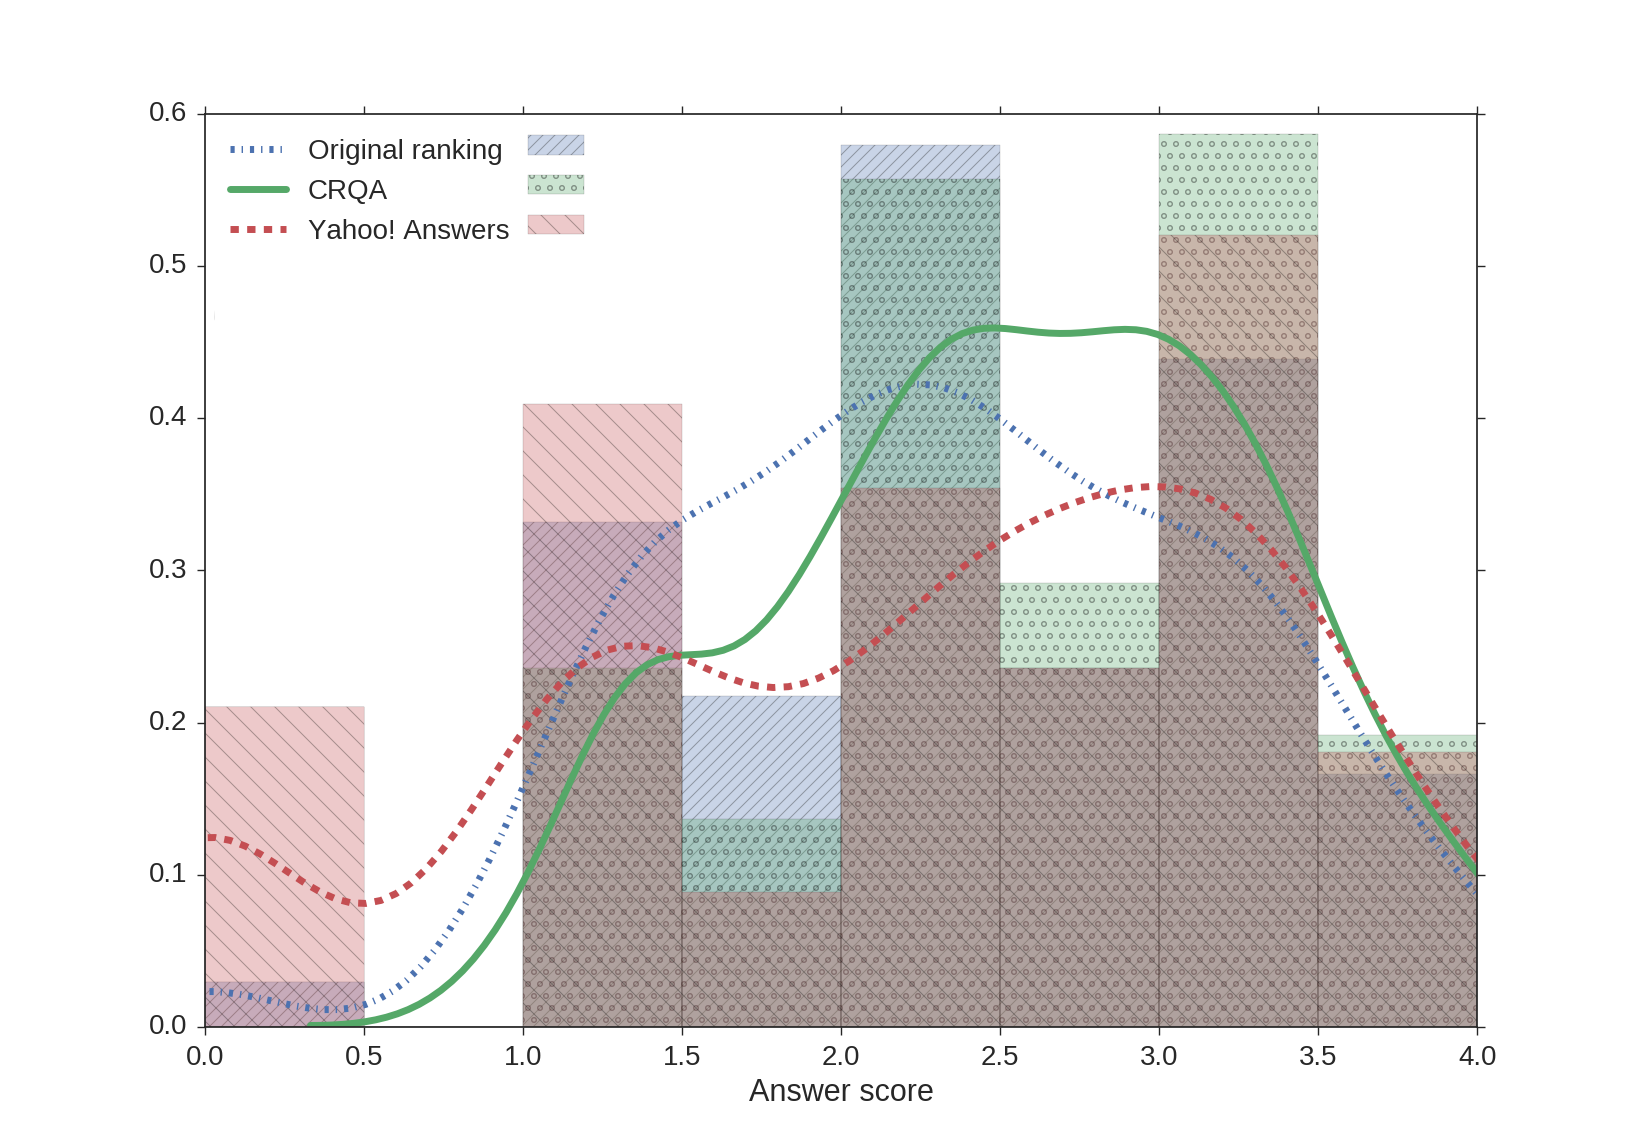
\includegraphics[width=0.5\textwidth]{img/score_hist}
	\caption{Histogram and kernel density estimation of answer scores for original candidate ranking, CRQA model re-ranking and Yahoo! Answers answers}
	\label{fig:score_histogram}
\end{figure}

Therefore, for RQ1 we can conclude, that crowdsourcing can effectively help automated QA system to improve the performance of question answering, by providing worker generated answers and rating existing candidates.

To summarize, our Crowd-powered Real-time Question Answering system substantially improves the quality compared to the baseline fully automated system, and generated answers are often even preferred to responses posted by CQA community.

\section{Analysis and Discussion}
\label{sec:analysis}

In this section we will analyze some of the results of our experiments and discuss their implications.

\subsection{Worker answers vs ratings}
\label{sec:analysis:answers_vs_ratings}

First, let's look at the contribution of additional answers and answer ratings provided by the workers.
These two types of contributions are complimentary to each other and attempts to solve different problems.
Table \ref{table:performance} shows the performance of our question answering system using each of these types of feedback independently.
The results demonstrate that both answers and ratings have positive effect on the performance.
Even with limited time, workers were able to reliably rate candidate answers, which helped the system to select a better final answer and improve the model precision.
However, this method doesn't help the system in cases, when it wasn't able to generate a good candidate in the first place, therefore using ratings only has lower average answer score than using worker generated answers.
By asking the crowd to provide a response if they can answer the question, CRQA covers this gap, which is important as in a real scenario even a fair answer would probably be better for the user than no answer at all.
Of course, given limited time and the fact that a random worker might not possess an expertise required to answer the question, such answers don't always perfectly answer the question.
\todo[inline]{One of the limitations of the paper is that it does not discuss the type of topics / questions on which the approach  works well and the type of topics on which the use of crowdsourcing fails.}
Table \ref{table:answer_examples} gives some examples of worker generated answers with low and high quality scores.

To summarize our answer to RQ2, ratings of answer candidates and worker generated answers both have similar positive effect on the performance of our question answering system.
What is more important, the contributions are independent and therefore it is beneficial to use both of them in the final system.

\begin{table*}[ht]
\centering
\begin{tabular}{| p{10.5cm} | p{5cm} | c |}
\hline
Question & Answer & Score \\
\hline
 Is Gotu Kola a good herb for mental health? How long does it take to work?? & yes & 1.66\\
 \hline
Can I write any number on line number 5 of a W2?  would like to set up my W2 were I get the most out of my paycheck and not have to pay taxes at the end of the year... & W2 & 1.33\\
 \hline
I need help with my mum? Something traumatic happened to me about 4 years ago i randomly asked my mother why when I lived with you in your home country a man that was our neighbour used to call me his daughter and the younger kids that lived there called me there cousins and one boy called me his sister? & yes & 1.0\\
\hline
\hline
 Is it bad not wanting to visit your family? & It's nt bad. Just be honest with them. They may be upset but they should understand & 3.0 \\
 \hline
Any health concerns with whey protein? So I workout 3-5 days a week and i drink a whey protein isolate after each workout. Since I workout almost everyday, is it ok for me to just drink a shake everyday?.. & As long as you use it as directed, there should not be any major problems.  You may want to consult your doctor just in case, but I would not be too concerned. & 3.0\\
\hline
Foot pain unable to walk? Hi so today woke with some pain, I'm able to put weight on my heel with no problem or pain.  But  the area between my heel and toes hurts really bad when I try to go with the motion of taking a step. Its not swollen and I don't remember hurting it at all & Possible gout in your foot, also possible you may have strained it during the previous day. & 3.0\\
\hline
What is a good remedy/medicine for stomach aches? Specifically ones caused by stress or anxiety? & Chamomile tea should help & 3.66\\
\hline
\end{tabular}
\caption{Examples of answers provided by the crowd workers and their average quality scores}
\label{table:answer_examples}
\end{table*}

\subsection{Selection of answer candidate for rating}
\label{sec:analysis:order}

Predicting the quality of answers and ranking them to select the best is one of the main challenges in automated question answering \cite{surdeanu2011learning}.
External feedback, such as noisy answer ratings, obtained from the crowd workers, provide valuable information, which, as our results demonstrate, can help a QA system to better re-rank the answers.
However, the capacity of crowdsourcing for answer ratings are obviously limited, as systems often are dealing with hundreds and thousands of answer candidates for a given question.
In this work, we made a choice to rate only top-7 answers according the automated system ranking.
This decision was made based on the average number of ratings workers could provide in the allotted time\footnote{The answers were posted for rating automatically after an automated system was done with candidate generation and ranking. On average users had $\sim$ 35 seconds to provide the ratings.}.
However, the order in which the answers are shown can also have a strong effect on the system performance, because the answers are typically rated one by one in the order they are displayed on the screen.
Our system included two strategies for answer ordering: random or according to their ranking score.
The former strategy provides a uniform coverage for all the answers selected for rating, while the later puts more emphasis on the currently top scoring candidates.
We randomly selected one of the strategies for each user and question.
To analyze the performance of each of the strategies we compute the average score of answers, generated using the corresponding ratings.
The average score for answers generating when candidates are shuffled is 2.508, and it's 2.539 when the candidates are sorted according to their model ranking score.
This suggests, that it's beneficial to allocate more of the workers attention on the top scoring candidate answers.

\subsection{Cost analysis}
\label{sec:analysis:cost}

The results of our experiments clearly demonstrated that crowdsourcing can improve the performance of near real-time question answering system.
The next reasonable question is what is the price of this improvement.
In our study we paid workers \$1.00 per single 15 minutes task, and each 15 minutes we had 10 assignments, which translates to \$15.00 per 15 minutes.
Overall, our experiment cost \$0.88 per question, and in this section we will discuss some ideas to reduce this cost.

First, we will study the effect of the number of workers on the performance of our CRQA system.
For this experiment we randomly sampled certain percentage of workers and removed all contributions (answers and ratings) of others.
Figure \ref{fig:nworkers_vs_quality} plots the dependency of the performance of our QA system on the number of workers.

\begin{figure*}[h!t]
  \begin{subfigure}[t]{0.5\textwidth}
	\centering
	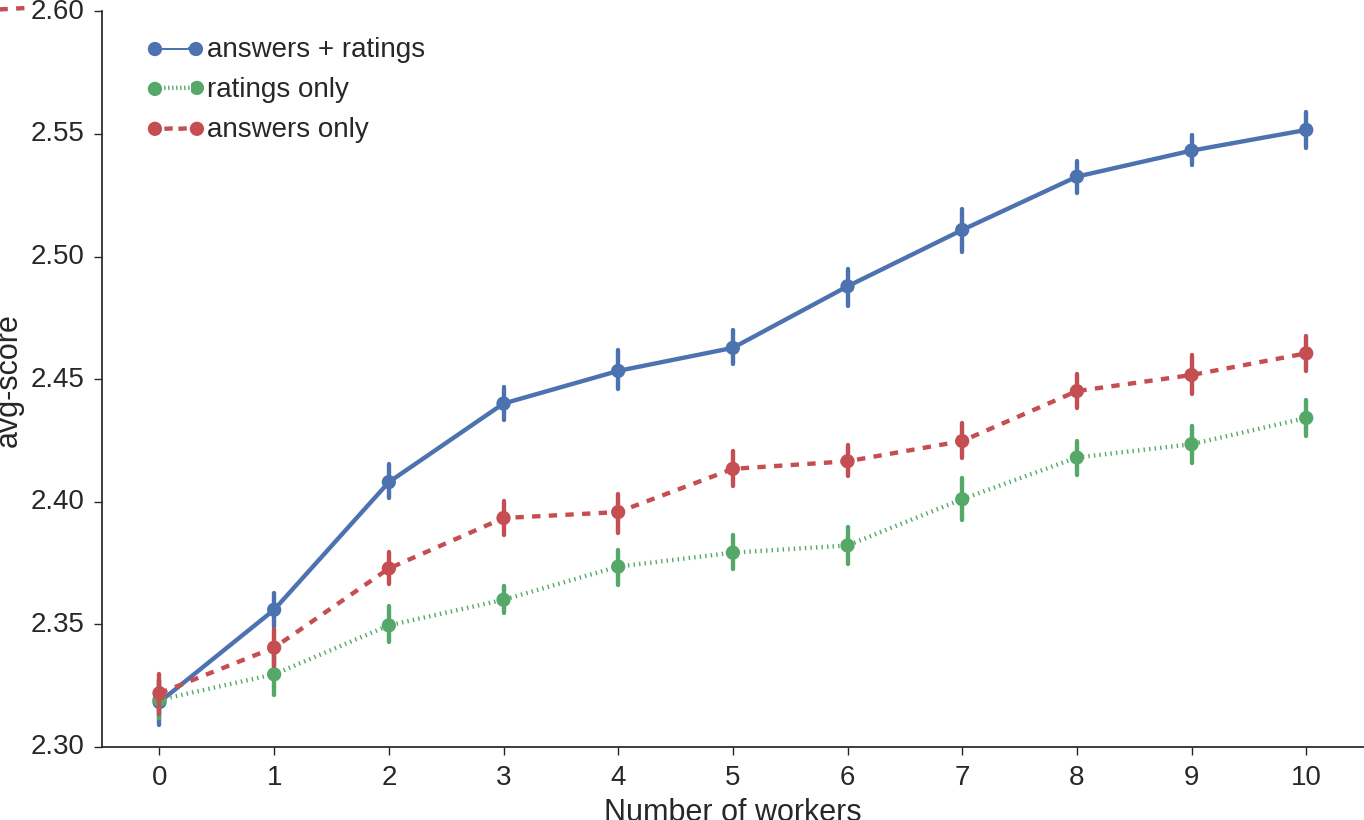
\includegraphics[width=\textwidth]{img/nworkers_vs_accuracy}
	\caption{avg-score: Average score per question}
	\label{fig:nworkers_vs_accuracy}
  \end{subfigure}
  \begin{subfigure}[t]{0.5\textwidth}
	\centering
	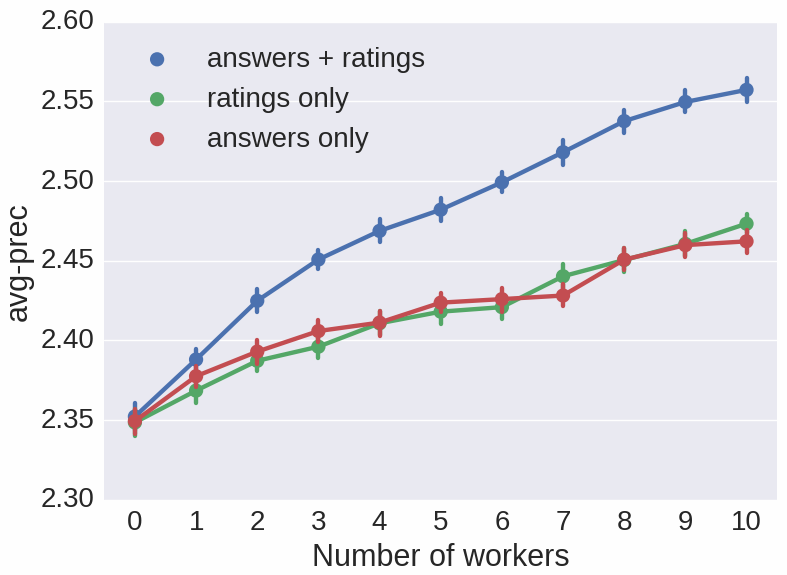
\includegraphics[width=\textwidth]{img/nworkers_vs_precision}
	\caption{avg-prec: Average score per answer (ignoring non-answered questions)}
	\label{fig:nworkers_vs_precision}
  \end{subfigure}
	\caption{Plot showing how the quality of the final answer depends on the number of workers per question}
	\label{fig:nworkers_vs_quality}
\end{figure*}

Obviously more workers mean more reliable answer ratings and more answer candidates, which improves the performance of the question answering system.
However, we can observe diminishing returns, as the cost per extra gain in performance metrics decreases as the number of workers grow.
Half of the overall performance improvement could be achieved with only 3 workers per question, which would save 70\% of the costs.

An alternative cost-reduction strategy is selective triggering of crowdsourcing, which would only ask for workers feedback for some of the questions.
Such a strategy would be necessary to scale a crowd-powered question answering system to a higher volume of questions.
There are multiple different approaches for such selective crowdsourcing: \textit{e.g.} a system can only ask for crowd contributions if it didn't generate enough candidate answers or the predicted quality of the top scoring candidates is low \cite{carmel2010estimating,he2006query}.
We leave this questions for the future work, as here we focused on the scenario, proposed by the organizers of the TREC LiveQA shared tasks, where questions arrive one by one and it's possible to utilize crowd input for every questions.

To summarize and answer RQ3, in the explored real-time QA scenario it is possible to reduce the costs of crowdsourcing by reducing the number of workers, although with some performance losses.
Our analysis suggests that paying 30\% of the original cost would give 50\% of the performance improvement.
% THE ANSWER IS KIND OF WEAK...

% \subsection{Time of day}
% Does the quality differ in different times of day?

\section{Related Work}
\label{sec:related_work}
Using the wisdom of a crowd to help users satisfy their information needs has been studied before in the literature.
\cite{bernstein2012direct} explored the use of crowdsourcing for offline preparation of answers to tail search queries.
Log mining techniques were used to identify potential question-answer fragment pairs, which were then processed by the crowd to generate the final answer.
This offline procedure allows a search engine to increase the coverage of direct answers to user questions.
In our work, however, the focus is on online question answering, which requires fast responses to the user, who is unlikely to wait more than a minute.
Another related work is targeting a different domain, namely SQL queries.
The CrowdDB system \cite{franklin2011crowddb} is an SQL-like processing system for queries, that cannot be answered by machines only.
In CrowdDB human input is used to collect missing data, perform computationally difficult functions or matching against the query.
In \cite{aydin2014crowdsourcing} authors explored efficient ways to combine human input for multiple choice questions from the ``Who wants to be a millionaire?'' TV show.
In this scenario going with the majority for complex questions isn't effective, and certain answerer confidence weighting schemas can improve the results.  
CrowdSearcher platform of \cite{Bozzon:2012:ASQ:2187836.2187971} proposes to use crowds as a data source in the search process, which connects a searcher with the information available through the users of multiple different social platforms.
In general, such websites open up many opportunities to interact with their users, in particular, identify users who might possess certain knowledge and request it by asking questions.
For example, \cite{nichols2012asking,nichols2013analyzing,mahmud2013recommending} showed that it's possible to get the information about airport security waiting times and product reviews by asking social network users, who identified themselves as being at an airport or mentioned the product of interest correspondingly.
While in this work, we primarily focused on more traditional way of hiring the crowd workers using Amazon Mechanical Turk, integration with social services is an interesting direction for the future work.

Many works have used crowdsourcing to get a valuable information that could guide an automated system for some complex tasks.
For example, entity resolution system of \cite{Whang:2013:QSC:2536336.2536337} asks questions to crowd workers to improve the results accuracy.
Using crowdsourcing for relevance judgments has been studied extensively in the information retrieval community, e.g., \cite{Alonso:2008:CRE:1480506.1480508,alonso2011design,grady2010crowdsourcing} to name a few.
The focus in these works is on document relevance, and the quality of crowdsourced judgments.
Whereas in our paper we are investigating the ability of a crowd to quickly assess the quality of the answers in a nearly real-time setting.
The use of crowdsourcing in IR isn't limited to relevance judgements.
The work of \cite{harris2013comparing} explores crowdsourcing for query formulation task, which could also be used inside an IR-based question answering system.
\cite{lease2013crowdsourcing} provides a good overview of different applications of crowdsourcing in information retrieval.

Crowdsourcing is usually associated with offline data collection, which requires significant amount of time.
Its application to (near) real-time scenarios poses certain additional challenges.
\cite{bernstein2011crowds} introduced the retainer model for recruiting synchronous crowds for interactive real-time tasks and showed their effectiveness on the best single image and creative generation tasks.
VizWiz mobile application of \cite{bigham2010vizwiz} uses a similar strategy to quickly answer visual questions.
This work builds on these ideas and uses the proposed retainer model to integrate a crowd into a real-time question answering system.
The work of \cite{Lasecki:2013:CCC:2501988.2502057} showed how multiple workers can sit behind a conversational agent named Chorus.
Similarly to this work, Chorus used crowd workers to propose and vote on responses to user messages.
However, our CRQA system represents a hybrid approach to question answering, where the automatic QA module proposes certain answer candidates, and workers can judge their quality as well as propose additional responses.
Such an approach allows us to focus on more complex informational questions, for many of which the workers might not know the answer, but still can contribute by estimating the quality of automatically generated candidates.
Chorus, on the contrary, considered somewhat simpler tasks (\textit{e.g.}, things to do in a new place, dinner date ideas, textit{etc.}), but focused more on maintaining a coherent dialog, which poses additional challenges, such as keeping a working dialog memory, keeping the users engaged with the dialog using gamification.
These ideas can be combined with the ideas of our work to build more intelligent assistants, that do not rely completely on the expertise of the workers.
Another use of a crowd for maintaining a dialog is presented in \cite{Bessho:2012:DSU:2392800.2392841}, who let the crowd handle difficult cases, when a system was not able to automatically retrieve a good response from the database of twitter data.
In our paper, we focus on a single part of the human-computer dialog, i.e. question answering, which requires a system to provide some useful information in a response to the user.

\section{Conclusion} 
In this paper we presented CRQA, the first, as far as we know, real-time question answering system that integrated crowd work within an automated QA system.
Specifically, we explore different methods of obtaining input from the crowd, and use a machine-learned answer re-ranking model that incorporates the crowd input as features to select the final system answer to return to the user. 

We report a large-scale experiment in which over a thousand real user questions were submitted to the CRQA system in real time, as part of the LiveQA challenge.
CRQA was able to successfully answer these questions in under 1 minute, with over 80\% of the answers subsequently rated to be fair or better.
Importantly, CRQA significantly improved question quality and coverage compared to the starting automated-only system, and, surprisingly, was able to return better answers on average compared to the traditional CQA system with millions of users (Yahoo! Answers) with answers collected more than \textit{two days} after the original posting time.

The described CRQA implementation is a promising step towards efficient and close integration of crowd work and automated analysis for real-time question answering.
It raises many promising issues and opens directions for future work, such as the performance of the crowdsourcing module when given less or more time to work, selective crowdsourcing for only the questions deemed ``difficult'' for the automated system; more efficient online learning for obtaining ratings from the crowd and integrating them into the ranking model; and investigating additional features and sources of evidence for improving the joint ranking of the system and crowd input.
This paper provides a flexible and powerful framework for combining the powers of crowdsourcing with automated question answering techniques, for building the next generation of real-time question answering systems.


\section{Acknowledgments}
The authors are grateful to the anonymous reviewers for their valuable comments and suggestions.
This work was partially supported by the Yahoo Labs Faculty Research Engagement Program (FREP).

\bigskip
\bigskip

\bibliographystyle{aaai}
\bibliography{references}

\end{document}
